\section{Scatterplot characterization}
\label{sec:visualizer:scatterplot}

\subsection{Characteristics of a ``good'' plot}
\label{sec:visualizer:scatterplot:goodplot}

The simplest scatterplot is the response against the observed variables. This, however, may not be the best way to ascertain independence for the user. This notion is illustrated in Figure~\ref{fig:visualizer:cdf}. The left plot appears to be independent as it’s a cluster of points near the origin, but it's not entirely clear due to the multitude of stray points around the concentrated section. By looking at the outliers, it could also be argued that there is some dependency. However, applying the CDF in both directions creates a plot distributed on (0,1). It should be noted that this transformation is non-destructive and preserves dependency in the data if it exists. The data is clearly independent as the points appear to be uniformly distributed within the plot.

\begin{figure}[htb]
	\begin{center}
		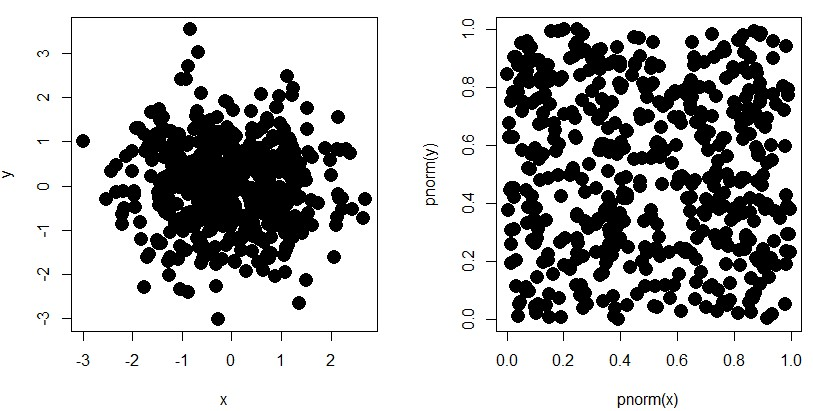
\includegraphics[width=0.75\linewidth]{ch-visualizer/figures/cdf}
		\caption[A plot of $y$ against $x$ after the CDF is applied in both directions.]{A plot of $y$ against $x$ with no transformation (left) and after the CDF is applied in both directions (right). The code for this example may be found in ~\ref{sec:appendicies:cdf}}
		\label{fig:visualizer:cdf}
	\end{center}
\end{figure}

Restricting the plot to a unit box allows analyst's visual systems to focus on locations where there is low spatial frequency, which is ideal for detecting dependence~\cite{hofert2016}. The effects of this can be progressively observed by looking from the left to the right in Figure~\ref{fig:visualizer:hofertoldford} below.

\begin{figure}[htb]
	\begin{center}
		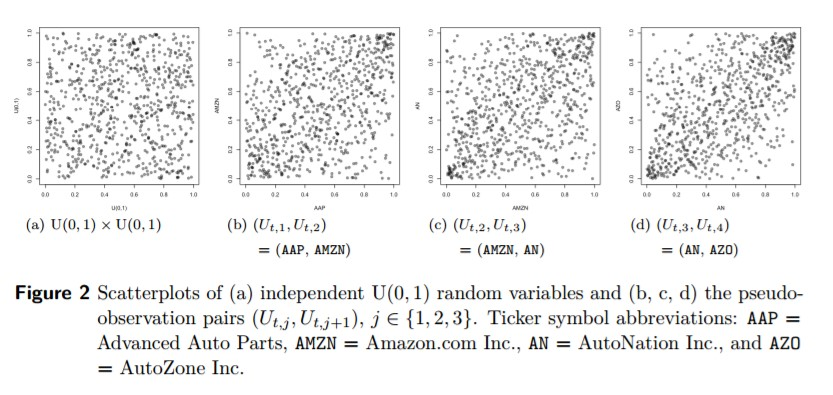
\includegraphics[width=0.75\linewidth]{ch-visualizer/figures/hofertoldford}
		\caption[Scatterplots of independent $U(0,1)$ random variables and the pseudo-observation pairs $(U_{t,j},U_{t,j+1}),j\in \{1,2,3\}$.]{Scatterplots of (a) independent $U(0,1)$ random variables and (b,c,d) the pseudo-observation pairs $(U_{t,j},U_{t,j+1}),j\in \{1,2,3\}$. Ticker abbreviations: AAP = Advanced Auto Parts, AMZN = Amazon.com Inc, AN = AutoNation Inc., AZO = AutoZone Inc. Images from Hofert and Oldford 2016~\cite{hofert2016}}
		\label{fig:visualizer:hofertoldford}
	\end{center}
\end{figure}

\subsection{Ordering}
\label{sec:visualizer:scatterplot:ordering}

As people interact with graphs, they maintain a ``mental map'' of the graph. Federico and Miksch note that the importance of the mental map depends on various factors such as the user preferences and tasks that they must complete~\cite{federico2016}. By ``mental map,'' Federico and Miksch mean that when users label a new graph, they remember the previous plots that they labeled~\cite{federico2016}. Supposing that the graphs that a program wants to show the user are already decided. Given a gradation of graphs (showing graphs that are most alike one after the other), users are less able to distinguish between differences than if they are shown graphs from different ends of the spectrum at different times~\cite{federico2016}. While their work primarily concerns itself with ordering graphs for interpretability, their results can be applied to scatter plots. To put it concisely, the scatter plot display itself is not the only thing that matter. The ordering of the display matters, as well, and it is best to show the plots in an order that allows users to distinguish the differences among graphs that they have already seen. By improving their understanding of the plots, careful display ordering advances the accuracy of user responses. User responses can be thought of as observations of the user’s true preferences, and the ordering of plots as a way to future tune the precision of the decision tree (Section~\ref{sec:visualizer:al}). 

\subsection{Conditional scatter plots}
\label{sec:visualizer:scatterplot:conditional}

((There are many ways to produce this scatter plot. One way is to marginally plot one explanatory variable against the response variable. We experiment with another way where, similar to regression, we control for the behavior of all the other explanatory variables while making this scatter plot. ))